\documentclass[aps,prl,twocolumn,superscriptaddress,floatfix]{revtex4-2}

\usepackage[T1]{fontenc}
\usepackage{lmodern}
\ifdefined\pdfgentounicode\input{glyphtounicode}\pdfgentounicode=1\fi
\usepackage{amsmath,amssymb,amsthm}
\usepackage{graphicx}
\usepackage{bm}
\usepackage{array}[=2016-10-06]
\usepackage{xcolor}
\definecolor{linkblue}{HTML}{1F5FBF}
\definecolor{citemagenta}{HTML}{C0157D}
\usepackage[colorlinks=true,linkcolor=linkblue,citecolor=citemagenta,urlcolor=linkblue]{hyperref}
\usepackage{orcidlink}
\hypersetup{pdftitle={The Fundamental Memory Ceiling of Noisy Quantum Reservoirs},pdfauthor={Markus Baumann, Jonas Stein, Claudia Linnhoff-Popien}}

\theoremstyle{plain}
\newtheorem{theorem}{Theorem}
\newtheorem{lemma}{Lemma}
\newtheorem{proposition}[lemma]{Proposition}
\newtheorem{corollary}[lemma]{Corollary}

\newcommand{\tr}{\operatorname{Tr}}
\newcommand{\ket}[1]{|#1\rangle}
\newcommand{\ketbra}[2]{|#1\rangle\!\langle #2|}
\newcommand{\nrm}[2]{\lvert #1\rvert_{#2}}
\newcommand{\Norm}[1]{\lVert #1\rVert}
\newcommand{\cD}{\mathcal D}
\newcommand{\cE}{\mathcal E}
\newcommand{\Nq}{\mathcal N_q}
\newcommand{\AD}{\mathcal{A\hspace{-0.6pt}D}}
\newcommand{\runin}[1]{\textit{\textbf{#1}}---}

\begin{document}

% The table of contents lists only the Supplemental Material: entries of the main text are not recorded.
\let\SMaddcontentsline\addcontentsline
\renewcommand{\addcontentsline}[3]{}

\title{The Fundamental Memory Ceiling of Noisy Quantum Reservoirs}

\author{Markus Baumann\,\orcidlink{0009-0007-3575-1006}}
\email[Contact author: ]{markus.baumann@campus.lmu.de}
\author{Jonas Stein\,\orcidlink{0000-0001-5727-9151}}
\author{Claudia Linnhoff-Popien\,\orcidlink{0000-0001-6284-9286}}
\affiliation{Quantum Applications and Research Laboratory (QAR-Lab),
Ludwig-Maximilians-Universit\"at M\"unchen, Oettingenstra\ss e 67, 80538 M\"unchen, Germany}

\date{October 19, 2026}

\begin{abstract}
Fresh qubits, not size, set how long a noisy quantum system can remember. With $k$ fresh qubits per time step, the longest memory under depolarizing noise is $\exp[\Theta(k)]$ time steps, whatever the size and unitary: keeping an input for $T$ steps needs $\Theta(\log T)$ fresh qubits per step, and that many suffice. A universal upper bound and an explicit reservoir that attains the scaling prove this for quantum reservoirs. The bound uses only the entropy budget of a time step and holds for any Markovian noisy dynamics with fresh qubits and no classical feedback, including measurement-free error correction.
\end{abstract}

\maketitle

%======================================================================
% MAIN TEXT
%======================================================================

\runin{Introduction.}Reservoir computing processes time series by injecting inputs into a fixed physical system and training only a linear readout~\cite{Jaeger2001,Maass2002,JaegerHaas2004,Lukosevicius2009,Tanaka2019}. Quantum reservoir computing (QRC) uses interacting qubits for this purpose~\cite{Fujii2017,Nakajima2019,Mujal2021} and has been realized on superconducting processors with up to 120 qubits~\cite{Chen2020,Suzuki2022,Yasuda2023,Hu2024,Monzani2024}. For temporal tasks, memory is the decisive resource. A reservoir can use an input only as long as that input still influences its state, and on noisy hardware this influence fades at every time step. Can a noisy quantum reservoir, or any noisy quantum system supplied with fresh qubits [Fig.~\ref{fig:scope}], remember arbitrarily far back, provided it is made large enough?

\begin{figure}[t]
\centering
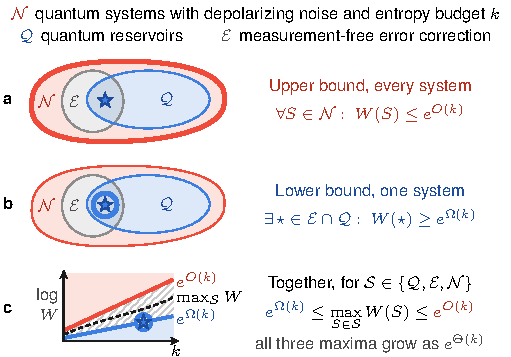
\includegraphics{fig1.pdf}
\caption{\textbf{Scope of the memory limit} (schematic).
(a)~The upper bound of Theorem~\ref{thm:main} holds for every system in $\mathcal N$: dynamics with Markovian depolarizing noise, $k$ fresh qubits per time step, and no classical feedback, whatever its size and gate set.
(b)~One explicit system (star) in $\mathcal E\cap\mathcal Q$, the error-correcting reservoir of Fig.~\ref{fig:attain}(a), attains the lower bound, so it bounds the largest memory in both sets from below.
(c)~Since $\mathcal Q,\mathcal E\subseteq\mathcal N$, all three maxima grow as $e^{\Theta(k)}$ at fixed noise and accuracy [Fig.~\ref{fig:limit}(a)].}
\label{fig:scope}
\end{figure}

\begin{figure*}[t]
\centering
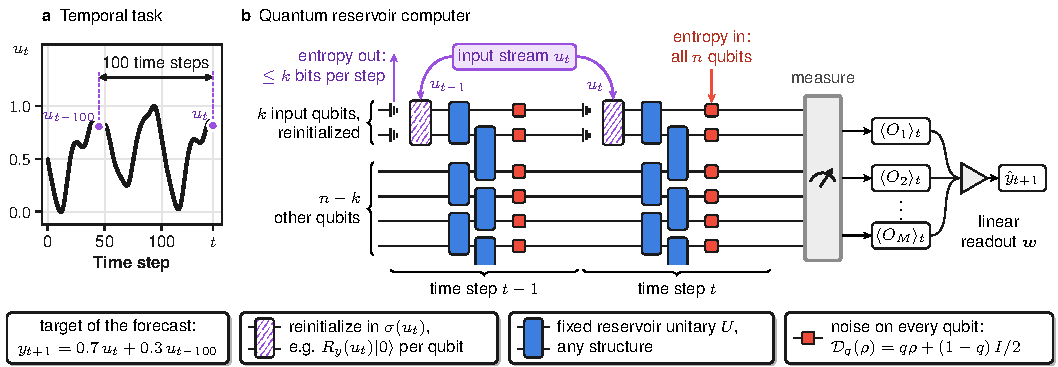
\includegraphics{fig2.pdf}
\caption{\textbf{Noisy quantum reservoir computing.}
(a)~Forecasting $y_{t+1}=0.7\,u_t+0.3\,u_{t-100}$ needs a memory of 100 time steps.
(b)~Every time step reinitializes $k$ input qubits in $\sigma(u_t)$, applies a fixed unitary $U$ to all $n$ qubits, and depolarizes every qubit; a linear readout predicts $\hat y_{t+1}$. Noise injects entropy into all $n$ qubits, but only the $k$ input qubits carry it out.}
\label{fig:overview}
\end{figure*}

The answer is not obvious. A larger reservoir can spread information about past inputs over more degrees of freedom, which promises robustness to noise. Refreshing matters too: QRC discards and reinitializes the input qubits at every time step, which removes accumulated entropy [Fig.~\ref{fig:overview}(b)]~\cite{Fujii2017,Yasuda2023,Hu2024}, while noise brings entropy into every qubit at every time step.

Fading memory is well studied: echo-state and fading-memory criteria guarantee that old inputs eventually lose their influence~\cite{Jaeger2001,Boyd1985,MartinezPena2023,MorguiSancho2026}, and Markovian reservoirs forget exponentially fast~\cite{Sannia2026}. Dissipation and resets are recognized resources for QRC~\cite{Chen2020,Kubota2023,Sannia2024,Monzani2024,Freiheit2026}, and in noisy quantum computation fresh qubits are indispensable, since without them depolarizing noise permits only logarithmically deep computations~\cite{Aharonov1996,BenOr2013,StilckFranca2021,Mele2026}. But how much memory a given supply of fresh qubits can buy has remained open.

The memory ceiling is set by fresh qubits, independently of size. Let $k$ input qubits be reinitialized at each time step, and let every qubit undergo depolarizing noise that keeps its state with probability $q$. The memory depth of a reservoir is the number of past inputs that still change its state by more than $\varepsilon$. The largest memory depth that any such reservoir can attain grows exponentially with $k$ and does not depend on the total number of qubits $n$ [Fig.~\ref{fig:limit}(a)]:
\begin{equation}
W_{q,k}(\varepsilon)=\exp\!\big[\Theta_q(k)\big]\quad\text{at fixed }\varepsilon.
\label{eq:main}
\end{equation}
That $O(\log T)$ fresh qubits per round suffice to keep a classical bit for $T$ rounds is the repetition code with majority vote~\cite{vonNeumann1956}. New is the converse, and it is universal within this noise model: $\Omega(\log T)$ fresh qubits per time step are necessary for any admissible dynamics, with or without code structure, and neither size nor entanglement nor the choice of unitary can substitute for them [Fig.~\ref{fig:limit}(b)]. Counting entropy does not give this, because a mixed state can still remember; the proof caps the purity of every reservoir state independently of $n$ and shows that noise erases every difference not backed by purity. Earlier limits on noisy computation bound the total number of physical qubits~\cite{Fawzi2022} or restrict the gate set to Clifford circuits~\cite{Nelson2026}. Theorem~\ref{thm:main} bounds the fresh-qubit rate instead, for any gate set and any system size~\cite[Sec.~VIII\,B]{SM}. Non-unital noise can replace fresh qubits~\cite{BenOr2013}, so the theorem charges it to the budget, and it requires a depolarizing component because dephasing alone can preserve a classical bit~\cite{SM}.

Because the upper-bound proof uses only the entropy budget of each noisy time step, it also bounds driven memory in other quantum architectures supplied with fresh qubits and without classical feedback, under the same local depolarizing-noise assumptions: input-driven variational quantum recurrent neural networks~\cite{Takaki2021}, repeated-interaction models with fresh ancillas~\cite{Cattaneo2021}, and dynamical circuits with resets~\cite{Yasuda2023,Hu2024}, including measurement-free error correction~\cite{Heussen2024}.

\runin{A reservoir with fresh qubits.}A reservoir of $n$ qubits receives one classical input $u_t$ per time step $t$ [Fig.~\ref{fig:overview}(a),(b)]. At each time step, the $k$ qubits of the input register are discarded and reinitialized in an input state $\sigma(u_t)$ that encodes the input. A fixed reservoir unitary $U$ then acts on all qubits. Finally, every qubit undergoes depolarizing noise $\cD_q(\rho)=q\rho+(1-q)\tr(\rho)I/2$. Altogether,
\begin{equation}
\rho_t=\cD_q^{\otimes n}\Bigl(U\bigl[\sigma(u_t)\otimes\tr_{\mathrm{in}}\rho_{t-1}\bigr]U^\dagger\Bigr),
\label{eq:model}
\end{equation}
where $\tr_{\mathrm{in}}$ is the partial trace over the input register. A trained linear readout turns the state into a prediction $\hat y_{t+1}=\sum_iw_i\tr(O_i\rho_t)=\tr(F\rho_t)$. This covers the original QRC proposal~\cite{Fujii2017} and protocols that measure and reset qubits without feedback~\cite{Yasuda2023,Hu2024}. We impose no restriction on $\sigma(u)$ or $U$; the unitary may even depend on the input.

The input qubits enter our analysis through a single number. Because $\sigma(u)\le I$, one time step can lower the entropy of a completely mixed reservoir by at most $k$ bits; formally, the map $\cE_u(X)=U[\sigma(u)\otimes\tr_{\mathrm{in}}X]U^\dagger$ obeys $\cE_u(I)\le2^kI$. We call $k$ the entropy \emph{budget} of a time step.

Noise erases the initial state, so the reservoir eventually reaches a state that depends only on the input history $h=(\dots,u_{t-1},u_t)$, its \emph{echo state} $\rho(h)$~\cite{Jaeger2001,MartinezPena2023,SM}. The \emph{memory depth} $W(\varepsilon)$ is the smallest number $L$ of time steps such that any two input histories that agree on their last $L$ inputs lead to echo states with $\tfrac12\Norm{\rho(h)-\rho(h')}_1\le\varepsilon$. Inputs older than $W(\varepsilon)$ change every linear readout by at most $2\varepsilon\Norm F$~\cite{SM}, so the memory depth, unlike the memory capacity~\cite{Jaeger2002}, limits all readouts at once. We write $W_{q,k}(\varepsilon)$ for the largest memory depth of any reservoir with $k$ input qubits, maximized over $n$, $U$, and $\sigma$.

\begin{figure*}[t]
\centering
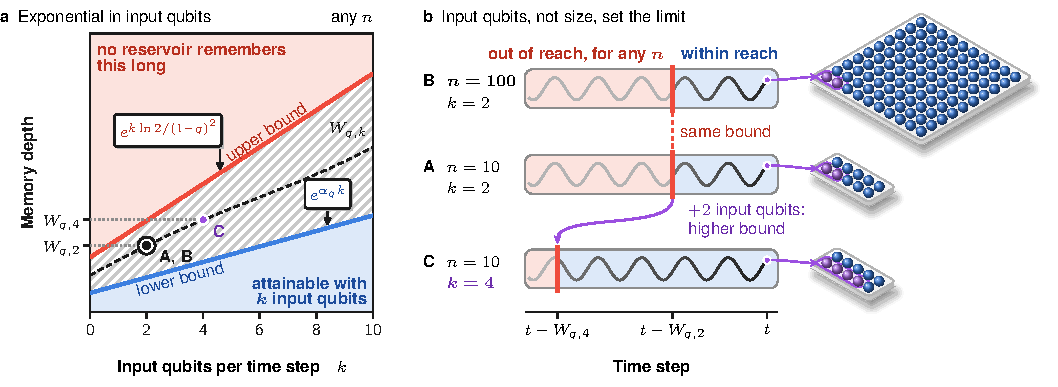
\includegraphics{fig3.pdf}
\caption{\textbf{The memory limit} (schematic).
(a)~The optimum over reservoir sizes lies between two exponentials in $k$ (Theorem~\ref{thm:main}); A, B, and C mark the reservoirs of (b).
(b)~One input stream drives three reservoirs: A and B differ tenfold in size but share $k=2$ input qubits, and C is A with two more input qubits. Inputs older than the bound (red) are out of reach for every reservoir with the same $k$, so A and B share the bound $W_{q,2}$, and C's bound $W_{q,4}$ lies further back.}
\label{fig:limit}
\end{figure*}

\runin{The memory limit.}Our main result bounds $W_{q,k}$ from both sides.

\begin{theorem}[Memory limit]\label{thm:main}
Let $0<q<1$.\\[2pt]
(i)~For $0<\varepsilon<1$, every reservoir with $k$ input qubits, whatever its number of qubits, reservoir unitary, and input encoding, has
\begin{equation}
W(\varepsilon)\le\Bigl\lceil\delta^{-1}\ln\frac1\varepsilon\Bigr\rceil,\qquad\delta^{-1}=2^{(1+4q)/(1-q)}\,2^{\beta_qk},
\label{eq:upper}
\end{equation}
with $\beta_q=q(1+q^2)/[(1-q)(1-q^2)]$, and \mbox{$\delta^{-1}\le2^{k/(1-q)^2}$} for $k\ge4$.\\[2pt]
(ii)~For $0<\varepsilon<q$ and every $k$ with $e^{\alpha_q(k-3)}\ge4$, there is a reservoir with at most $2k$ qubits that has
\begin{equation}
W(\varepsilon)\ge\tfrac14\,e^{\alpha_q(k-3)}\ln\frac q\varepsilon ,
\label{eq:lower}
\end{equation}
where $\alpha_q=\frac12\ln\frac1{1-q^2}$.
\end{theorem}

At fixed noise strength and accuracy, both bounds are exponential in $k$ and independent of $n$: the fresh-qubit rate sets the optimal memory scaling. One explicit reservoir attains the lower bound [Fig.~\ref{fig:scope}], while the upper bound covers every reservoir; neither size nor entanglement nor the choice of unitary can change this scaling class. The two exponents differ, so the theorem fixes the class but not the exact rate~\cite[Sec.~III\,G]{SM}. For readouts of finite precision, the upper bound carries over to the memory capacity~\cite{SM,Jaeger2002}.

The upper bound uses the reservoir only through its budget: any channel with $\cE(I)\le2^kI$ may replace the injection step, resets and measurement-free recovery operations included~\cite{SM}. The theorem concerns echo states: a larger reservoir needs a longer washout of its initial state, $\Theta_q(\log n)$ time steps for $n$ redundant copies of a bit~\cite{SM}, without raising the ceiling for driven memory.

\runin{Why no reservoir can remember longer.}A proof must defeat every strategy a reservoir might use to hide information: spreading it over many qubits, entangling it, or using its input qubits for repair. Ours follows the difference between two reservoir states with different input histories and asks how well the states can be distinguished and how concentrated their difference is. Two properties of depolarizing noise~\cite{King2014,Cubitt2015} answer both and yield the bound in three steps.

\emph{Step 1: Noise caps the purity.} We measure the purity of a state by $\log_2P^2=n-S_2(\rho)$, the number of pure qubits' worth of purity it holds, where $S_2$ is the R\'enyi-2 entropy. Depolarizing noise damps the many-qubit correlations of which purity is made; this is hypercontractivity~\cite{King2014}. As a result, every time step multiplies the log-purity by $\theta=2q^2/(1+q^2)<1$, while the input qubits add at most $\theta k$. In a reservoir of any size, every echo state therefore holds at most $\log_2P_*^2=2kq^2/(1-q^2)$ pure qubits' worth, about 8.5 per input qubit at $q=0.9$~\cite{SM}.

\emph{Step 2: Spread-out differences are erased.} Low purity alone does not mean forgetting: $\ketbra00\otimes I/2^{n-1}$ and $\ketbra11\otimes I/2^{n-1}$ are almost completely mixed, yet perfectly distinguishable. Their difference, however, is spread over the whole Hilbert space, and one layer of noise erases the fraction $1-q$ of their distinguishability. Reverse hypercontractivity makes this precise~\cite{Cubitt2015}: noise forces two states to overlap unless their difference is concentrated, so one layer of noise erases a fixed fraction of every spread-out difference.

\emph{Step 3: Concentration costs purity.} A distinguishable difference concentrated on a fraction $2^{-m}$ of the Hilbert space, such as a bit stored in $m$ redundant copies, requires about $m$ pure qubits' worth of purity, and Step~1 caps the purity. A distance $V$ that weighs distinguishability against concentration~\cite{SM} therefore shrinks at every time step $\Phi_u$, for any two reservoir states $\rho,\rho'$ and any input $u$:
\begin{equation}
V\bigl(\Phi_u\rho-\Phi_u\rho'\bigr)\le(1-\delta)\,V(\rho-\rho'),
\label{eq:contraction}
\end{equation}
with the forgetting rate $\delta$ of Eq.~\eqref{eq:upper}~\cite{SM}. Whatever the reservoir does, every time step erases at least the fraction $\delta$ of its past. After $L$ time steps, two echo states are therefore within trace distance $e^{-\delta L}$; this is Theorem~\ref{thm:main}(i).

Without fresh qubits ($k=0$), as for inputs encoded in input-dependent unitaries, the echo state is completely mixed for every input sequence, so such a reservoir retains nothing~\cite{Aharonov1996,SM}.

\begin{figure*}[t]
\centering
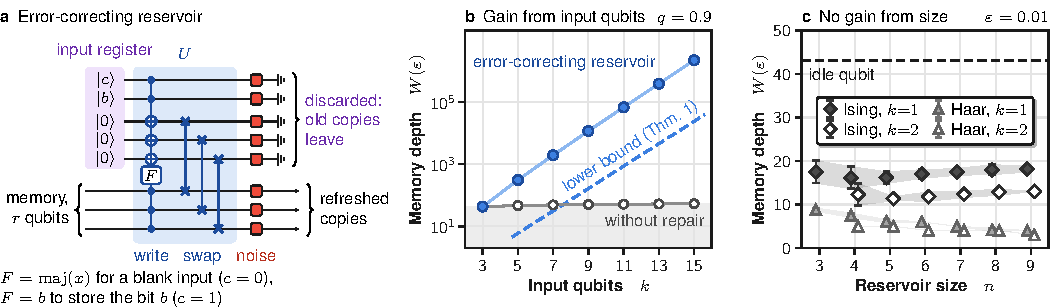
\includegraphics{fig4.pdf}
\caption{\textbf{Attaining the limit.}
(a)~Error-correcting reservoir ($r=3$, $k=5$): $U$ writes the new bit, or the majority of the stored copies, into fresh ancillas and swaps them into the memory; the old copies leave with the input register.
(b)~The error-correcting reservoir (exact single-qubit readout, $n=2k-2$) uses its fresh qubits for repair, and its memory depth grows exponentially with $k$, above the lower bound of Theorem~\ref{thm:main}; without repair (gray), the same $r=k-2$ copies gain almost nothing, even with the best readout. Plotted depths are continuous threshold crossings; integer depths are rounded up.
(c)~Within the sampled ensembles, standard reservoirs gain nothing from size, and a second input qubit shortens their memory ($k=1$ filled, $k=2$ open; mean $\pm$ s.d., six realizations). Unitaries are sampled separately for each $k$. (b),~(c)~$q=0.9$, $\varepsilon=0.01$.}
\label{fig:attain}
\end{figure*}

\runin{A reservoir that attains the limit.}A single reservoir suffices to attain the optimal scaling of $W_{q,k}$; it may be classical because the upper bound covers every quantum reservoir. Our exactly solvable error-correcting reservoir repairs its memory with fresh qubits [Fig.~\ref{fig:attain}(a)]. It stores a bit in $r$ memory qubits as a repetition code and corrects it by majority vote~\cite{vonNeumann1956}. At every time step, its unitary computes the majority of the stored copies, writes it into $r$ freshly reinitialized ancillas, and swaps the ancillas into the memory. The old copies, which carry the noise, end up in the input register and are discarded at the next injection, so the entropy leaves with them. Two further input qubits tell the reservoir whether to keep its memory or to store a new bit, so that $k=r+2$~\cite{SM}. The unitary only permutes computational basis states: the construction is classical reversible logic run on qubits, and it is measurement-free error correction~\cite{Heussen2024} in its simplest form.

Because all states remain diagonal, every qubit behaves as a classical bit that flips with probability $(1-q)/2$ per time step, and the response can be computed exactly. The stored bit is lost only if most of its $r$ copies flip within one time step, which happens with probability $p_r\le(1-q^2)^{r/2}=e^{-\alpha_qr}$ by a Chernoff bound with the exact exponent~\cite{SM}. A bit $b$ stored $t$ time steps ago therefore leaves every memory qubit with
\begin{equation}
\langle Z\rangle_t=(-1)^b\,q\,(1-2p_r)^t .
\label{eq:response}
\end{equation}
The signal still decays, but at a rate that is exponentially small in $r$. Two input histories that differ only in this bit agree on their last $t$ inputs, yet their echo states remain at trace distance at least $q(1-2p_r)^t$; with the bound on $p_r$, this gives Theorem~\ref{thm:main}(ii). At $q=0.9$ and $\varepsilon=0.01$, the single-qubit memory depth exceeds 300 time steps for $k=5$ and two million for $k=15$. For the odd values $k=5,\ldots,15$ in Fig.~\ref{fig:attain}(b), each pair of additional input qubits increases this depth by more than a factor of five. The same copies without majority vote keep the bit for at most 53 time steps; the fresh qubits extend memory because the reservoir uses them for repair.

\runin{Standard reservoirs operate far below the limit.}The simulations do not test the bound; they locate standard reservoirs relative to it. We simulated transverse-field Ising reservoirs with random all-to-all couplings, the workhorse of QRC~\cite{Fujii2017,Nakajima2019,MartinezPena2021}, and Haar-random unitaries at $q=0.9$, and estimated their memory depth $W$ at $\varepsilon=0.01$~\cite{SM}. Within these ensembles, size does not extend their memory [Fig.~\ref{fig:attain}(c)]. With one input qubit ($k=1$), the Ising reservoir remembers 16 to 18 time steps for every size from $n=3$ to $9$ qubits, while the Haar reservoir forgets faster as it grows ($W$ drops from 9 to 4 time steps). Nor do more input qubits help [Fig.~\ref{fig:attain}(c)]~\cite{SM}. At fixed size ($n=8$), raising $k$ from 1 to 4 lowers $W$ from 18 to 8 time steps (Ising) and from 4 to 3 (Haar), and the decrease persists when the additional input qubits are reinitialized in $\ket0$. Both stay below an idle qubit that merely holds the input ($W=43$ time steps), whereas the error-correcting reservoir of the same size ($n=8$, $k=5$) remembers over 300 time steps.

\runin{Beyond reservoirs: an entropy budget.}For other noise, the result becomes an entropy budget~\cite{SM}. Any additional channel $\mathcal S$ with $\mathcal S(I)\le2^bI$ adds $b$ bits, and the upper bound holds with $k$ replaced by $k+b$. Unital noise (Pauli errors, dephasing, coherent errors, crosstalk) and projective measurements whose outcomes only enter the readout~\cite{Mujal2023} have $b=0$; since every unital qubit channel with full-rank Choi matrix contains a depolarizing component, the theorem covers generic independent unital noise~\cite{SM}. Resets of $m$ qubits count like $m$ input qubits. Amplitude damping with probability $0<\gamma<1$ adds $n\log_2(1+\gamma)$ bits, and relaxing idle qubits then act as a refrigerator~\cite{BenOr2013} that lets a reservoir with two input qubits remember for a time exponential in $n$~\cite{SM,Hoeffding1963}. In the language of error correction, a measurement-free recovery that consumes $k$ fresh ancillas per round is, with its data qubits, a system in $\mathcal N$ [Fig.~\ref{fig:scope}]: it keeps a logical bit for at most $\exp[O_q(k)]$ rounds beyond the washout of its initial state, whatever its size, and feedback of syndromes into a classical memory, outside the model, can lift this ceiling~\cite{SM}. Without a depolarizing component or with non-Markovian noise~\cite{Sannia2026}, memory can likewise be unbounded~\cite{SM}.

\runin{Conclusion.}Under the stated noise model, the fresh-qubit supply sets the memory ceiling; reaching its scaling requires dynamics that uses those qubits to remove errors. Fresh qubits are necessary to reach the memory limit but not sufficient; standard reservoirs, which do not use them for repair, operate far below it. The limit bounds how far back a task can reach; how well a reservoir processes the inputs within that range is a separate question~\cite{Cao2026}. Open problems include closing the gap between the two exponents, whether a quantum code can beat the classical rate $\alpha_q$, what limits memory with feedback or non-Markovian noise, and testing the scaling by varying $k$ at fixed $n$ with mid-circuit resets~\cite{Yasuda2023,Hu2024}.

\begin{acknowledgments}
\runin{Acknowledgments.}Claude Opus 5.5 (Anthropic) assisted with manuscript preparation, checks of derivations and references, and simulation and plotting code. Markus Baumann reviewed the outputs and takes responsibility for the final content.
\end{acknowledgments}

\runin{Data availability.}Code and data that reproduce all numbers and figures are provided with the Supplemental Material~\cite{SM}.

% References cited only in the Supplemental Material (through the note of Ref. SM); the \nocite lets a single
% BibTeX run of the Letter alone find them, with the same numbering.
\nocite{Xiong2025,Dao2026}
\bibliography{refs}

\end{document}
